\chapter{Protótipo da Interface de Modelagem}
\label{cp:prototipo}

Neste capítulo é apresentada a interface da implementação parcial (situação atual do desenvolvimento) tanto da camada de interface para modelagem gráfica quanto da camada de persistência para a notação.
Primeiramente, em relação à camada de interface, trata-se de uma plataforma \textit{web} e, para sua implementação, foram utilizados a linguagem de marcação HTML 5 (\textit{HyperText Markup Language}), o CSS 3 (\textit{Cascading Style Sheets}) e a linguagem \textit{JavaScript}. Adicionalmente, as bibliotecas \textit{JQuery} e \textit{SVGPanZoom} são utilizadas para facilitar a implementação de recursos gráficos e execução de requisições HTTP/Ajax para a comunicação com o servidor, e manipulação dos elementos gráficos por meio de de operações de escala e deslocamento, respectivamente.

A ferramenta foi projetada para ser simples e intuitiva, com foco na elaboração dos diagramas. A página inicial é apresentada na Figura~\ref{inicial}.

\begin{figure}[!htb]
\centering
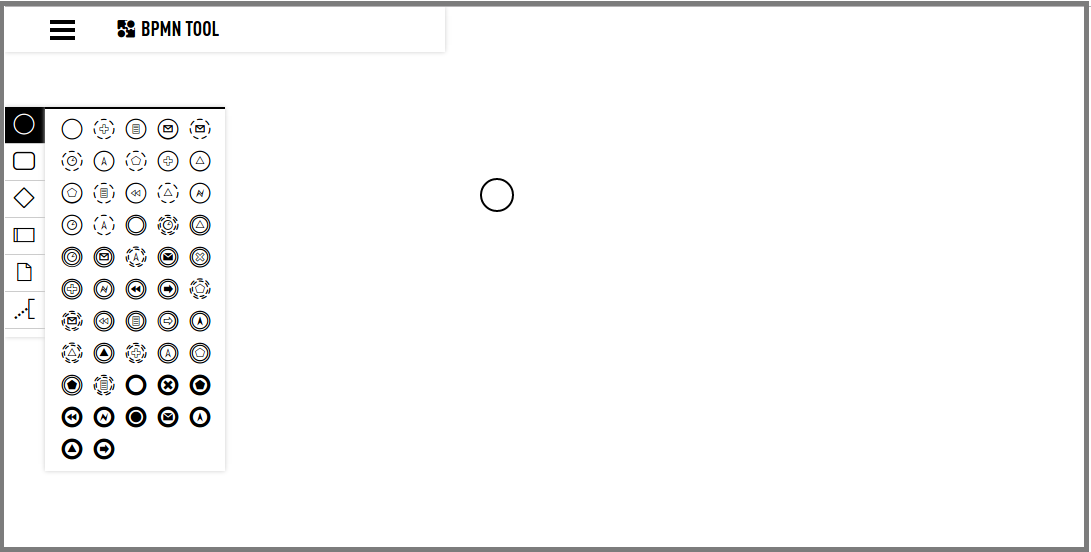
\includegraphics[width=\textwidth]{images/ferramenta.png}
\caption{Interface de modelagem da notação.}
\label{inicial}
\end{figure}

Para a criação de um novo modelo de diagrama de processo de negócio, é necessário somente realizar a inserção dos componentes do diagrama, ou caso já haja um modelo representado, o usuário deve selecionar a opção \textit{"Menu -> New"} para iniciar a representação. O menu da ferramenta é apresentado na Figura~\ref{menu}.

\begin{figure}[!htb]
\centering
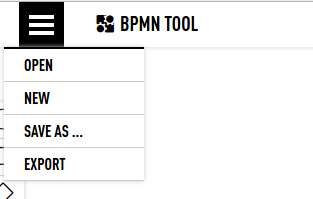
\includegraphics[scale=0.75]{images/menu.png}
\caption{Menu de opções da ferramenta.}
\label{menu}
\end{figure}

Ainda em relação à Figura~\ref{menu}, é possível observar outras opções. Na opção \textit{``Menu -> Open''}, o usuário abrir um modelo de processo de negócio elaborado previamente nesta ferramenta, armazenados em arquivos com a extensão \textit{.bpmn}. A opção ``\textit{Menu -> Save as''} permite o armazenamento do modelo no mesmo formato citado anteriormente, sendo este um diagrama concluído ou em processo de criação. Por fim, a opção \textit{``Menu -> Export''} visa armazenar o modelo em formato de imagem vetorial, no formato SVG (\textit{Scalable Vector Graphics}), de forma que, o usuário, mesmo sem acesso a esta ferramenta, possa ter acesso ao conteúdo do modelo, ao menos, para leitura de seu conteúdo.

Para a construção do modelo de processo de negócio, o usuário faz uso de elementos tais como: \textit{Events}, \textit{Gateways}, \textit{Tasks}, \textit{Pools/Lanes}, \textit{Data Objects} e \textit{TextAnnotations}. Estes elementos são encontrados na ferramenta pelo menu lateral, no qual estão presentes todos os itens dessa categorias listas anteriormente.

Na Figura~\ref{eventos}, todos os eventos e suas derivações são listados.

\begin{figure}[!htb]
\centering
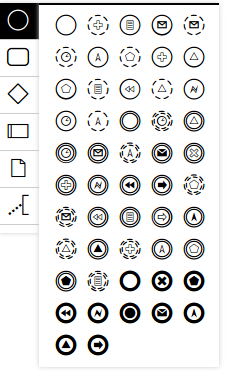
\includegraphics[scale=0.75]{images/eventos.png}
\caption{Painel de elementos da categoria de eventos.}
\label{eventos}
\end{figure}

Na Figura~\ref{gate} são apresentados os elementos que compõem a categoria de portões. E na Figura~\ref{lane} são exibidos os elementos referentes a piscinas e raias.

\begin{figure}[!htb]
\centering
\subfigure[Categoria de \textit{gateways}\label{gate}]{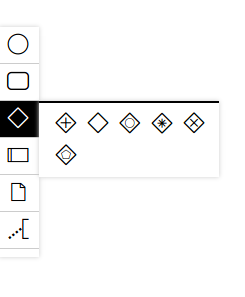
\includegraphics[scale=0.75]{images/gate.png}}\qquad\qquad
\subfigure[Categoria de piscinas e raias\label{lane}]{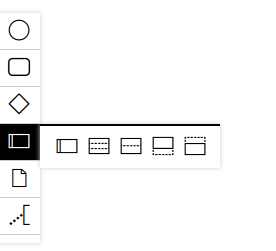
\includegraphics[scale=0.75]{images/lane.png}}
\caption{Painel de elementos}
\label{elementos}
\end{figure}
%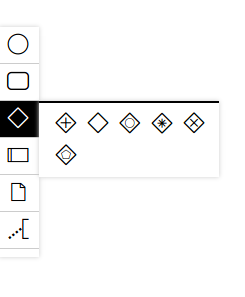
\includegraphics[scale=0.75]{images/gate.png}




Cada elemento pertencente à notação será persistido no formato XML para composição do pacote de laboratório. A figura~\ref{mensagem} representa uma tarefa da categoria de mensagens, este elemento será armazenamento no modelo apresentado na listagem~\ref{ls:message}

\begin{figure}[!htb]
\centering
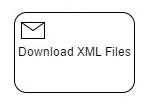
\includegraphics[scale=0.75]{images/mensagem.jpg}
\caption{Exemplo de elemento \textit{MessageTask}.}
\label{mensagem}
\end{figure}

\lstset{language=XML}
\begin{lstlisting}[caption=Descrição do elemento \textit{Mensagem}, label=ls:message]
<messagetask id="23">
	<type>task</type>
	<from>15</from>
	<to>42</to>
	<value>Download XML Files</value>
</messagetask>
\end{lstlisting}

Em relação ao servidor da plataforma \textit{web} em desenvolvimento, está sendo utilizada a linguagem de programação \textit{Java}, o servidor \textit{GlassFish Server 4.1} e o JSP - \textit{Java Server Pages}. Adicionalmente, para o suporte à serialização dos dados no formato XML (\textit{eXtensible Markup Language}) é utilizada a biblioteca \textit{XStream}. Esta parte da aplicação provê suporte tanto à leitura e escrita dos arquivos, quanto à validação dos diagramas, em termos de completude e corretitude, e também a extração do conteúdo de pacotes de laboratório e criação do respectivo modelo de processo. Aliás, a estrutura do arquivo XML deverá conter tanto elementos para representar o modelo visual BPMN (como coordenadas para posicionamento de elementos gráficos na interface), quanto elementos que representam os conceitos do Pacote de Laboratório.

Atualmente, em relação à camada de persistência, todos os elementos compõem a primeira versão da notação já foram implementados, e está em andamento a implementação dos elementos da segunda versão da notação BPM. Atualmente, foram implementadas trinta e uma classes, divididas em seis pacotes conforme a categorização dos elementos da notação. Tem sido adotada uma abordagem evolutiva, portanto os diagramas, assim como o modelo de classes, têm sido, também, alvo de contante evolução.


A seguir, na Listagem\ref{lst:classe} é apresentada a classe \textit{BusinessProcessDiagram} (apenas dados privados, que devem ser armazenados), a qual representa o componente básico de um diagrama BPMN, sendo responsável pela organização de todo o diagrama. O armazenamento desse elemento em pacote de laboratório está representado na Listagem~\ref{xml}.

\lstset{language=java}
\begin{lstlisting}[caption=Estrutura de Dados inicial da classe diagrama BPM, label=lst:classe]
public class BusinessProcessDiagram {
    private String id; 
    private String name; 
    private String version; 
    private String author; 
    private String language;  
    private String queryLanguage; 
    private Date creationDate;
    private Date modificationDate; 
    private ArrayList<Pool> pools; 
    private String documentation; 
}
\end{lstlisting}


\lstset{language=XML}
\begin{lstlisting}[caption=Estrutura do XML da classe diagrama BPM, label=xml]
<businessprocessdiagram id="1245" name="Selecao dos grupos">
  <author>Leandro Ungari</author>
  <language>pt-br</language>
  <queryLanguage>BPMN</queryLanguage>
  <creationDate>01/05/2017</creationDate>
  <modificationDate>10/05/2017</modificationDate>
  <pools>
    <pool id="1">...</pool>
    <pool id="2">...</pool>
    <pool id="3">...</pool>
         ...
    <pool id="n">...</pool>
  </pools>
  <documentation>Elemento formalizado pela documentacao BPMN 2.0 ...
	</documentation>
</businessprocessdiagram>
\end{lstlisting}




